%%%%%%%%%%%%%%%%%%%%%%%%%%%%%%%%%%%%%%%%%
% Beamer Presentation
% LaTeX Template
% Version 1.0 (10/11/12)
%
% This template has been downloaded from:
% http://www.LaTeXTemplates.com
%
% License:
% CC BY-NC-SA 3.0 (http://creativecommons.org/licenses/by-nc-sa/3.0/)
%
%%%%%%%%%%%%%%%%%%%%%%%%%%%%%%%%%%%%%%%%%

%----------------------------------------------------------------------------------------
%     PACKAGES AND THEMES
%----------------------------------------------------------------------------------------
% !TeX TXS-program:compile = txs:///pdflatex/[--shell-escape]
\documentclass{beamer}
\usepackage[ngerman]{babel}


\mode<presentation> {

% The Beamer class comes with a number of default slide themes
% which change the colors and layouts of slides. Below this is a list
% of all the themes, uncomment each in turn to see what they look like.

%\usetheme{default}
%\usetheme{AnnArbor}
%\usetheme{Antibes}
%\usetheme{Bergen}
%\usetheme{Berkeley}
%\usetheme{Berlin}
%\usetheme{Boadilla}
%\usetheme{CambridgeUS}
%\usetheme{Copenhagen}
%\usetheme{Darmstadt}
%\usetheme{Dresden}
%\usetheme{Frankfurt}
%\usetheme{Goettingen}
%\usetheme{Hannover}
%\usetheme{Ilmenau}
%\usetheme{JuanLesPins}
%\usetheme{Luebeck}
\usetheme{Madrid}
%\usetheme{Malmoe}
%\usetheme{Marburg}
%\usetheme{Montpellier}
%\usetheme{PaloAlto}
%\usetheme{Pittsburgh}
%\usetheme{Rochester}
%\usetheme{Singapore}
%\usetheme{Szeged}
%\usetheme{Warsaw}

% As well as themes, the Beamer class has a number of color themes
% for any slide theme. Uncomment each of these in turn to see how it
% changes the colors of your current slide theme.

%\usecolortheme{albatross}
%\usecolortheme{beaver}
%\usecolortheme{beetle}
%\usecolortheme{crane}
%\usecolortheme{dolphin}
%\usecolortheme{dove}
%\usecolortheme{fly}
%\usecolortheme{lily}
%\usecolortheme{orchid}
%\usecolortheme{rose}
%\usecolortheme{seagull}
%\usecolortheme{seahorse}
%\usecolortheme{whale}
%\usecolortheme{wolverine}

%\setbeamertemplate{footline} % To remove the footer line in all slides uncomment this line
%\setbeamertemplate{footline}[page number] % To replace the footer line in all slides with a simple slide count uncomment this line

%\setbeamertemplate{navigation symbols}{} % To remove the navigation symbols from the bottom of all slides uncomment this line
}

\usepackage{graphicx} % Allows including images
\usepackage{booktabs} % Allows the use of \toprule, \midrule and
% \bottomrule in tables
\usepackage{listings}
\usepackage{parcolumns}
\usepackage[nocenter]{qtree}
\usepackage{minted}
\usepackage{eurosym}
\usepackage{qrcode}
\usepackage{xcolor}
\definecolor{LightGray}{gray}{0.95}
%----------------------------------------------------------------------------------------
%     TITLE PAGE
%----------------------------------------------------------------------------------------

\title[]{Einstieg in Latex} % The short title appears at the bottom of every slide, the full title is only on the title page

\author{Jules Kreuer} % Your name
\institute[FSI] % Your institution as it will appear on the bottom of every slide, may be shorthand to save space
{
	FSI Uni Tübingen\\
	aufbauend auf den Workshop von Adreas Rist 2019\\ % Your institution for the title page
	\medskip
	\textit{fsi@fsi.uni-tuebingen.de}\\
}
\date{14. Oktober 2021} % Date, can be changed to a custom date

\begin{document}

\begin{frame}
\titlepage % Print the title page as the first slide
\end{frame}

%----------------------------------------------------------------------------------------
%     PRESENTATION SLIDES
%----------------------------------------------------------------------------------------

%------------------------------------------------



\begin{frame}[fragile]
\frametitle{Was kann denn Latex?}
\[
\prod^6_{i=1} \frac{1}{2}i^2 + \pi
\]
\begin{minted}{python}
x = 1
for i in range(6):
	x = x*1/2*i**2 + pi
\end{minted}
Lorem ipsum dolor sit amet, consetetur sadipscing elitr,sed diam nonumy eirmod tempor invidunt ut labore et dolore magna aliquyam erat, sed diam voluptua.\\
....etc.
\end{frame}

\begin{frame}
\frametitle{Was ist Latex?}
     Latex ist also eine freeware Version von Word?\pause $\Rightarrow$ Nein, besser!
     
\end{frame}


\begin{frame}
     \frametitle{Was ist Latex?}
     \begin{columns}[c] % The "c" option specifies centered vertical alignment while the "t" option is used for top vertical alignment
          
          \column{.2\textwidth} % Left column and width
     \includegraphics[width=\textwidth]{pictures/texicon.png}
          \column{.1\textwidth} % Left column and width
     \Huge{$ \Rightarrow $}
          
          \column{.2\textwidth} % Right column and width
     \includegraphics[width=\textwidth]{pictures/pdficon.png}
          
     \end{columns}
\begin{itemize}[<+->]
     \item Datei wird in *.tex geschrieben
     \item *.tex wird in eine PDF umgewandelt
\end{itemize}
\end{frame}

\begin{frame}
     \frametitle{Du hast umgewandelt gesagt?}
     \begin{itemize}[<+->]
          \item Ja! Du wirst einen Compiler brauchen
               \item mkLatex, \textbf{pdfLaTeX}, XeLaTeX and LuaLaTeX
               \item Unter Windows: MikTex
     \end{itemize}
\end{frame}




\begin{frame}
     \frametitle{Wie geht das?}
     Keine Sorge! Es gibt tolle Editoren:
     \begin{itemize}[<+->]
          \item \textbf{Overleaf}
          \item \textbf{TexStudio}
          \item Sublime 
          \item Atom
          \item vim
     \end{itemize}
\end{frame}

\begin{frame}
	\frametitle{Overleaf}
	
\includegraphics[width=6cm]{pictures/overleaf.png}
	\begin{itemize}[<+->]
		\item Freemium online Editor und Compiler
		\item Gruppenfunktion
		\item Gut für kleinere Projekte (Übungsblätter)
	\end{itemize}
\end{frame}


\begin{frame}
	\frametitle{Overleaf}
	\centering
	\qrcode{https://www.overleaf.com?r=35c51bcf&rm=d&rs=b}\\
	\url{https://www.overleaf.com?r=35c51bcf}\footnote{Refferal link}
\end{frame}

\begin{frame}
	\frametitle{TexStudio}
	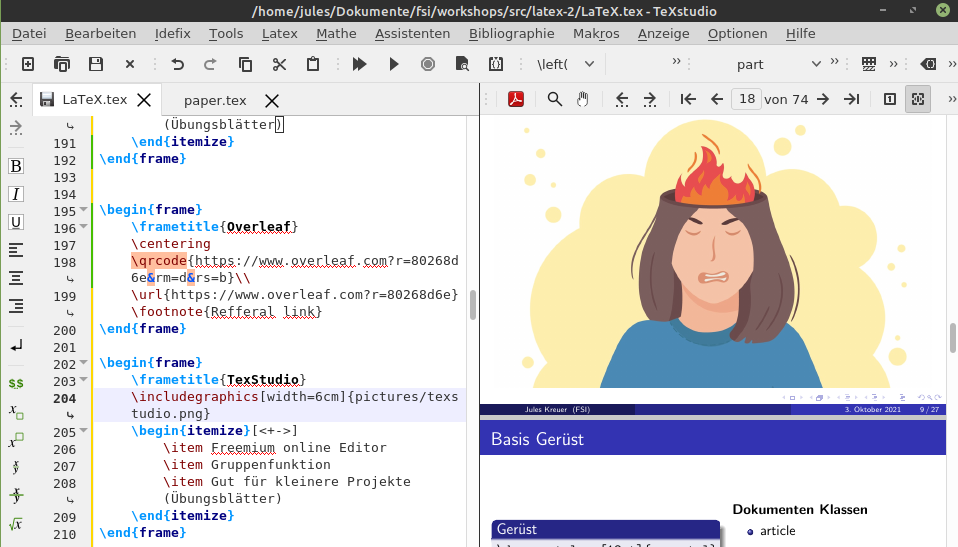
\includegraphics[width=6cm]{pictures/texstudio.png}
	\begin{itemize}[<+->]
		\item Offline Editor, benötigt Compiler
		\item keine Gruppenfunktion
		\item Compiler: ``nervige'' Installation von Paketen
		\item Danach: Gut für alle Projekte (Übungsblätter / BA / ...)
	\end{itemize}
\end{frame}

\begin{frame}[fragile]
	\frametitle{Compiler}
	Windows\vspace{2mm}
	\centering
	
	\qrcode{https://miktex.org/download}\\
	\url{https://miktex.org/download}\\
	\vspace{5mm}
	\hline
	\vspace{5mm}
	Linux
	\begin{minted}{bash}
	sudo apt install texlive-latex-extra # 0.5GB oder
	sudo apt install texlive-full        # 5.9GB
	\end{minted}
\end{frame}

\begin{frame}[fragile]
	\frametitle{TexStudio}
	Windows\vspace{2mm}
	\centering
	
	\qrcode{https://www.texstudio.org/}\\
	\url{https://www.texstudio.org/}\\
	\vspace{5mm}
	\hline
	\vspace{5mm}
	Linux
	\begin{minted}{bash}
sudo add-apt-repository ppa:sunderme/texstudio
sudo apt update
sudo apt install texstudio
\end{minted}
\end{frame}

\begin{frame}
\frametitle{Wann kommen wir endlich zum Coden?}
\includegraphics[width=\linewidth]{pictures/anger.jpg}
\end{frame}


\begin{frame}[fragile]
  
\frametitle{Basis Gerüst}
\begin{columns}
	\column{.5\textwidth}\begin{block}{Gerüst}
		
\begin{minted}{latex}
\documentclass[12pt]{scrartcl}
\usepackage[ngerman]{babel}
\usepackage[utf8]{inputenc}
% weitere imports...
\begin{document}
	(Inhalt)
\end{document}
\end{minted}
	\end{block}
	\column{.45\textwidth}
	\textbf{Befehle}
	\begin{itemize}[<+->]
		\item beginnen mit \textbackslash
		\item \% Kommentare
		\item \mintinline{latex}{\begin{..}} Umgebung
	\end{itemize}
\end{columns}
\end{frame}

\begin{frame}[fragile]
	\frametitle{Basis Gerüst}
	\begin{columns}
		\column{.5\textwidth}\begin{block}{Gerüst}
\begin{minted}{latex}
\documentclass[12pt]{scrartcl}
\usepackage[ngerman]{babel}
\usepackage[utf8]{inputenc}
% weitere imports...
\begin{document}
     (Inhalt)
\end{document}
\end{minted}
     \end{block}
          \column{.45\textwidth}
          \textbf{Dokumenten Klassen}
          \begin{itemize}[<+->]
               \item article
               \item letter
               \item scrartcl 
               \item exam
          \end{itemize}\pause
     \textbf{Wichtigste Imports}
     \begin{itemize}[<+->]
          \item mathtools,amsthm,amssymb
          \item fancyhdr
          \item graphicx
     \end{itemize}
          
     \end{columns}
\end{frame}

\begin{frame}[fragile]
\frametitle{Header und Footer}
\begin{columns}
\column{.39\textwidth}

\begin{block}{}
     \begin{minted}{latex}
(...)
\usepackage{fancyhdr}
\pagestyle{fancy} 
\fancyhf{} 
\fancyhead[L]{Titel} 
\fancyhead[C]{}           
\fancyhead[R]{Name}           
\fancyfoot[C]{\thepage}  
\begin{document}
    (...)
\end{document}
          \end{minted}
     \end{block}
\column{0.5\textwidth}
\begin{figure}

\begin{example}
\includegraphics[width=\linewidth,trim= 0cm 20cm 0cm 0cm,]{pictures/asdf0.pdf}

\end{example}\end{figure}
\end{columns}

\end{frame}

\begin{frame}[fragile]
	\frametitle{Header und Footer}
	\begin{columns}
		\column{.39\textwidth}
		
		\begin{block}{}
			\begin{minted}{latex}
(...)  
\begin{document}
\author{Jules Kreuer}
\title{Übungsblatt 0}
\date{\today{}}
\maketitle{}
(...)
\end{document}
\end{minted}
		\end{block}
		\column{0.5\textwidth}
		\begin{figure}
			
			\begin{example}
				
\includegraphics[width=\linewidth,trim= 4cm 23cm 4cm 1cm,]{pictures/uebung00.pdf}
				
		\end{example}\end{figure}
	\end{columns}
	
\end{frame}

%------------------------------------------------

\begin{frame}[fragile]
     \frametitle{Strukturierung und Nummerierung}
     \begin{columns}
          \column{.5\textwidth}
     \begin{block}{Kapitel}<1->
          \begin{minted}{latex}
\section{Sektion}
\subsection{SSektion}
\subsubsection{SSSektion}
\section*{Sektion}
          \end{minted}          
     \end{block}
     
\begin{block}{Aufzählung}<3->
     \begin{minted}{latex}
\begin{enumerate}
     \item Bla bla bla
     \item Mr Freeman
     \item here 
\end{enumerate}
     \end{minted}
     
\end{block}
\column{.45\textwidth}
\begin{example}
\includegraphics[width=\linewidth,trim=0cm 20cm 10cm 0cm]{pictures/asdf2.pdf}
\end{example}

\end{columns}
\end{frame}

\begin{frame}[fragile]
     \frametitle{Strukturierung und Nummerierung}
     \begin{columns}
     \column{.45\textwidth}
     
     \begin{block}{Stichpunkte}
          \begin{minted}{latex}
\begin{itemize}
    \item Bla bla bla
    \item Mr Freeman
    \item here 
\end{itemize}
          \end{minted}
      \end{block}
      \column{.45\textwidth}
      \pause
      \begin{example}
      \includegraphics[width=\linewidth,trim=1cm 18cm 10cm 0cm]{pictures/asdf3.pdf}
      \end{example}
     
     
     \end{columns}

\end{frame}

\begin{frame}[fragile]
     \frametitle{Euch gefällt die Nummerierung nicht?}
     
     \begin{columns}
     \column{0.45\textwidth}
     \begin{block}{andere Nummerierungen}
               
          \begin{minted}{latex}
\usepackage{enumerate}
\usepackage[shortlabels]
{enumitem}
(...)
\begin{enumerate}[a)]
    \item
     \item 
     \item[5]
\end{enumerate}
          \end{minted}
          \end{block}

     \column{0.45\textwidth}
          \begin{example}
                \includegraphics[width=\linewidth,trim= 0cm 10cm 0cm 0cm]{pictures/asdf4.pdf}
          \end{example}
     \end{columns}



\end{frame}

\begin{frame}[fragile]
\frametitle{Wie füge ich Bilder ein?}
\begin{block}{}
     \begin{minted}{latex}
\usepackage{graphicx}
(...)
\includegraphics[width=\linewidth]{pictures/balu.png}
     \end{minted}
\end{block}
\begin{example}
     \includegraphics{pictures/balu.jpg}
\end{example}

\end{frame}

\begin{frame}[fragile]
\frametitle{Wie gebe ich Bildern Untertitel?}
\begin{block}{}
     \begin{minted}{latex}
\begin{figure}
\centering
\includegraphics{pictures/balu.jpg}
\caption{Balu}
\end{figure}
     \end{minted}
     
\end{block}
\begin{example}\begin{figure}
     \centering
     \includegraphics[height=.3\textheight]{pictures/balu.jpg}
     \caption{Balu}
\end{figure}

\end{example}
\end{frame}


\begin{frame}[fragile]
\frametitle{Referenzen}
Label und Referenzen die anklickbar sind. 
\begin{block}{}
		\begin{minted}{latex}
Wichtige Aussage \label{key} \\
Referenz \ref{key}
\end{minted}
	\end{block}	
\end{frame}

\begin{frame}[fragile]
     \frametitle{Tabellen}
\begin{example}
     \begin{table}
          \begin{tabular}{l||c |r}
               Nummer& Schulden & Person der Schuld \\\hline
               1& 10\euro & Mirco \\
               2& 100\euro &Fachschaft\\
               3&1000\euro & Kuchen\\
          \end{tabular}
     \caption{Schuldentablle}

     \end{table}
\end{example}

\end{frame}

\begin{frame}[fragile]
\frametitle{Tabellen}
     \begin{block}{}
          \begin{minted}{latex}
\begin{table}
    \begin{tabular}{l||c |r}
        Nummer& Schulden & Person der Schuld \\\hline
        1& 10\euro & Mirco \\
        2& 100\euro &Fachschaft\\
        3&1000\euro & Kuchen\\
    \end{tabular}
\caption{Schuldentablle}
\end{table}
               
          \end{minted}
     \end{block}
\end{frame}

\begin{frame}
	\frametitle{Recap}
	\begin{alertblock}{Aufgabe}
		Erstellt folgendes Dokument in \LaTeX:
		
\includegraphics[width=7cm]{pictures/uebung.png}
	\end{alertblock}
\end{frame}

\begin{frame}
\frametitle{Mathematikumgebungen}
\begin{itemize}[<+->]
\item Inline: $\sum_{1}^{100}i=5050$ schreiben
\item Schöner:
\[ \sum_{1}^{100}i=\frac{100(100+1)}{2}=5050 \]
in einer neuen Zeile, damit unsere tolle Formel auch auffällt
\item Längere Formeln:
\begin{align*}
\sum_{k=1}^{n}2k&=2\cdot\sum_{k=1}^{n} k\\
&=2\cdot\frac{n(n+1)}{2}\\
&=n(n+1) = n^2+n
\end{align*}
\end{itemize}

\end{frame}

\begin{frame}[fragile]
\frametitle{Hinter der Mathemagie!}
\begin{block}{}
\begin{minted}{latex}
 $\sum_{1}^{100}i=5050$
\end{minted} 
\end{block}
\pause
\begin{example}
$\sum_{1}^{100}i=5050$
\end{example}
\pause
\begin{block}{}
\begin{minted}{latex}
\[ \sum_{1}^{100}i=\frac{100(100+1)}{2}=5050 \]
\end{minted}
\end{block}
\pause
\begin{example}
\[ \sum_{1}^{100}i=\frac{100(100+1)}{2}=5050 \]
\end{example}

\end{frame}
\begin{frame}[fragile]
\frametitle{Align Umgebung}
\begin{block}{}
\begin{minted}{latex}
\begin{align*}
    \sum_{k=1}^{n}2k&=2\cdot\sum_{k=1}^{n} k\\
                    &=2\cdot\frac{n(n+1)}{2}\\
                    &=n(n+1) = n^2+n
\end{align*}
\end{minted}
\end{block}
\begin{example}
\begin{align*}
    \sum_{k=1}^{n}2k&=2\cdot\sum_{k=1}^{n} k\\
                    &=2\cdot\frac{n(n+1)}{2}\\
                    &=n(n+1) = n^2+n
\end{align*}
\end{example}
\end{frame}
\begin{frame}
	\frametitle{Symbole}
	\centering
	\Large $\delta, \sigma, \xi, \cdot, \lambda, \not\subset, \leq, \ntrianglerighteq, ...$\\
	\vspace{5mm}
	\qrcode{https://oeis.org/wiki/List\_of\_LaTeX\_mathematical\_symbols}\\
	\normalsize
	\url{https://oeis.org/wiki/List_of_LaTeX_mathematical_symbols}
\end{frame}
\begin{frame}[fragile]
	\begin{alertblock}{Aufgabe}
		\begin{align*}
			\Delta  &= \lim\limits_{x \rightarrow 5} \lambda + \frac{1}{5-x}\\
			\nabla   &= \sqrt[3]{3\sigma}
		\end{align*}
	\end{alertblock}
	\pause
	\begin{block}{}
	\begin{minted}{latex}
\begin{align*}
  \Delta  &= \lim\limits_{x \rightarrow 5} \lambda 
	         + \frac{1}{5-x}\\
  \nabla   &= \sqrt[3]{3\sigma}
\end{align*}
\end{minted}
\end{block}
\end{frame}
\begin{frame}[fragile]
\frametitle{Hast du Klammern gesagt?}
Natürlich gibt es Probleme beim Klammern setzen!\\
\[f(x)=(\sum_{k=1}^{n}\underbrace{\frac{5(x+3)}{5}}_{=x+3})+g(x)\]\pause
"HEY! Das sieht blöd aus!"\pause Keine Sorge das geht besser!\\
\[f(x)=\left(\sum_{k=1}^{n}\underbrace{\frac{5(x+3)}{5}}_{=x+3}\right)+g(x)\]\pause
\begin{example}
\begin{minted}{latex}
\[f(x)=\left(
\sum_{k=1}^{n}\underbrace{\frac{5(x+3)}{5}}_{=x+3}
\right)
+g(x)\]
\end{minted}
\end{example}


\end{frame}

\begin{frame}[fragile]
\frametitle{ja gut... aber }
"Was ist mit dem Text über dem Gleichzeichen?"\pause
Meinst du vielleicht?
\[(a+b)^2\overset{ausm.}{=} a^2+2ab+b^2\]
\begin{example}
\begin{minted}{latex}
\[(a+b)^2\overset{ausm.}{=} a^2+2ab+b^2\]
\end{minted}
\end{example}
\end{frame}

\begin{frame}[fragile]
	\frametitle{Cheat Sheet}
	\begin{tabular}{c|l}
		math-mode	& \mintinline{latex}{$ ... $ oder \begin{align} ... \end{align}}\\
		Gruppen  & \mintinline{latex}{{ }}\\
		$\frac{x}{y}$ & \mintinline{latex}{\frac{x}{y}} \\
		$x^a_b$ & \mintinline{latex}{x^a_b} \\
		$\sum_{1}^{2}$ & \mintinline{latex}{\sum_{1}^{2}}\\
		$\sqrt[3]{x}$ & \mintinline{latex}{\sqrt[3]{x}}\\
		$\prod_{1}^{2}$ & \mintinline{latex}{\prod_{1}^{2}}\\
		$\leq \neq \geq$ & \mintinline{latex}{\leq \neq \geq}\\
		$\lim\limits_{x \rightarrow 5}$ & \mintinline{latex}{\lim\limits_{x \rightarrow 5}} \\
		$x_\text{text}$ &  \mintinline{latex}{x_\text{text}}}
		
		
	\end{tabular}
	
	
	\pause
	\begin{alertblock}{Aufgabe}
		\[\int_{a}^{b}\left( \sum^b_{\omega = 1}f(\omega)+g(x)\right)dx=\int_{a}^{b}\sum^b_{\omega = 1}f(\omega)dx+\int_{a}^{b}g(x)dx\]
	\end{alertblock}
	
\end{frame}


\begin{frame}[fragile]
\frametitle{Graphen und Bäume?}
\begin{itemize}[<+->]
\item yWorks yed (\url{https://www.yworks.com/products/yed-live})
\begin{itemize}
\item[+] Einfach zu Bedienen 
\item[+] Sehr mächtig
\item[-] man bekommt nur SVG oder anderes Bildformat
\end{itemize}
\item FSM Designer
\begin{itemize}
\item http://madebyevan.com/fsm/
\item[+] yeah man bekommt tex code
\item[-] code nicht gut lesbar
\end{itemize}
\end{itemize}\pause
$\Longrightarrow$ Geht das auch in händisch?

\end{frame}
\begin{frame}[fragile]
\frametitle{Bäume}
\begin{itemize}[<+->]
\item \textbf{qtree}\\
\Tree [.VP \qroof{this}.DP [.V$'$ is \qroof{a tree}.DP ] ]
\begin{minted}{latex}
\Tree [.VP \qroof{this}.DP [.V$'$ is \qroof{a tree}.DP ]]
\end{minted}
\item \textbf{tikz}
\end{itemize}

\end{frame}

\begin{frame}[fragile]
\frametitle{Pseudocode?}
\begin{itemize}[<+->]
\item verbadim
\begin{itemize}
\item klein und gut!
\end{itemize}
\item lstlisting
\begin{itemize}
\item eher geignet für Code der direkt aus einem File importiert wird
\item Syntaxhighlighting
\item Konfigurationsmöglichkeiten ohne Ende
\end{itemize}
\item pseudocode
\begin{itemize}
\item Sehr gut für Algorithmen
\end{itemize}
\item \textbf{minted}
\begin{itemize}
	\item gutes Syntaxhighlighting
	\item einfacher als lstlisting
	\item \begin{minted}[fontsize=\footnotesize]{python}
% !TeX TXS-program:compile = txs:///pdflatex/[--shell-escape]
	\end{minted}
\end{itemize}
\end{itemize}
\end{frame}


\begin{frame}
\frametitle{Tools}
\begin{itemize}
\item \url{https://www.tablesgenerator.com/}
\item \url{http://detexify.kirelabs.org/classify.html}
\item \url{https://mathpix.com/}
\end{itemize}
\end{frame}

\begin{frame}
	\frametitle{Vorlagen}
	\centering
	\qrcode{https://sandbox.fsi.uni-tuebingen.de/\~jules/latex-vorlagen/}\\
	\url{https://sandbox.fsi.uni-tuebingen.de/\~jules/latex-vorlagen/}
\end{frame}

\begin{frame}[fragile]
	\frametitle{}
	\begin{alertblock}{Aufgabe}
		Erstellt folgenden Inhalt:
		\begin{figure}
			\includegraphics[width=4cm]{pictures/balu.jpg}
			\caption{Balu Caption}
		\end{figure}
		\begin{minted}[bgcolor=LightGray]{python}
print("Example")
for i in range(0,5):
	i = i+1
\end{minted}
	\end{alertblock}
\end{frame}
\begin{frame}
	\centering
	\qrcode{https://juleskreuer.eu/projekte/latex/files/LaTeX.pdf}\\
	\url{https://juleskreuer.eu/projekte/latex/files/LaTeX.pdf}
\end{frame}

\end{document} 